% ----------------------- Project Planning -----------------------------------

\section{Project Planning}

\begin{comment}
    State your project plan with up-to-date tasks, dependencies, timelines and milestones. You may paste your plan appropriately from MS Project etc. 
\vspace{.1in}

\noindent
Include cost analysis if applicable. 
\vspace{.1in}

\noindent
Mention the software life cycle model you followed.    
\end{comment}

\subsection{Software Life Cycle Model}
\noindent
The project utilized an Iterative Waterfall model, combining structured progression with flexibility for revisions. This approach allowed revisiting earlier phases, such as refining requirements or enhancing data preprocessing, based on insights from analysis or testing. Feedback loops between phases ensured continuous improvement, fostering a robust system for detecting mental health disorders in social media posts while adapting to dynamic project needs.
\vspace{1em}

% Insert SDLC Images
\begin{figure}[h!]  
    \centering
    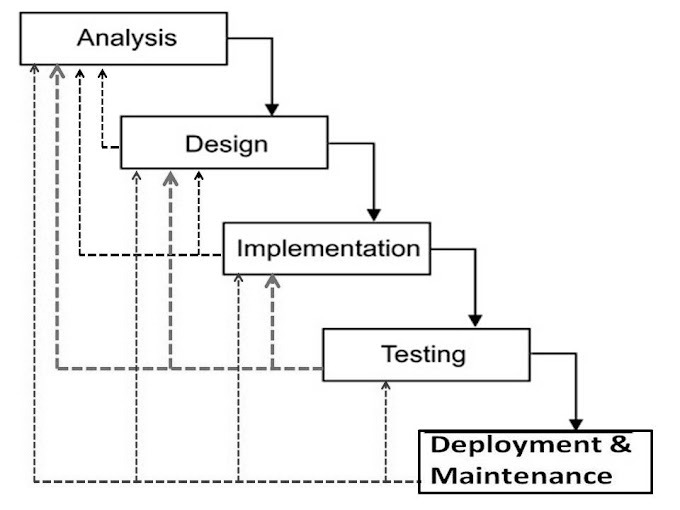
\includegraphics[width=0.6\textwidth]{Images/01 Life_cycle.jpg}  
    \caption{Iterative Waterfall Model}
    \label{Iterative Waterfall Model}  % Label for referencing the figure
\end{figure}

\noindent
The different phases are as follows:

\begin{itemize}
    \item \textbf{Requirement Gathering and Analysis} :
    \noindent
    This initial phase involved understanding the project's goals, objectives, and stakeholder expectations.
    \item \textbf{Data Collection and Preparation} :
    \noindent
    Utilizing Reddit API, the data collection phase was executed. This included downloading the dataset, examining its structure, and performing data cleaning and prepossessing to ensure its suitability for analysis.
    \item \textbf{Model Development} :
    \noindent
    This phase included the creation of a Bag of Words model, splitting the dataset into training and test sets, and implementing various machine learning algorithms.
    \item \textbf{Model Evaluation} :
    \noindent
    Following model development, testing and validation of the models were done, ensuring they met the required accuracy benchmarks. This phase involved using performance metrics such as accuracy, precision, recall, and F1-score to evaluate the models' effectiveness.
    \item \textbf{Final Deployment and Documentation} :
    \noindent
    The last phase focused on deploying the best-performing model and creating comprehensive documentation. This included user manuals and technical documentation to facilitate future maintenance and enhancements.
\end{itemize}


\subsection{Dependencies and Milestones} 
\noindent
Key dependencies were identified for successful project progression. For instance, completion of the data preparation phase was critical before proceeding to model development. Milestones were established at the end of each phase to ensure accountability and track progress. The successful completion of the requirement gathering phase marked the first milestone, followed by the data preparation phase, and so on.

\subsection{Scheduling}
\noindent
Effective scheduling is vital for project success. A detailed timeline with tasks like requirement gathering, data preprocessing, model implementation, and testing was created, with flexibility for adjustments based on feedback. Key milestones, including data analysis, model validation, and user acceptance testing, ensure progress tracking. Using tools like Microsoft Project, we monitor tasks, manage resources, and maintain communication to deliver a high-quality solution on time.

\pagebreak

% Insert MS Project Plan Image
\begin{figure}[h!]  
    \centering
    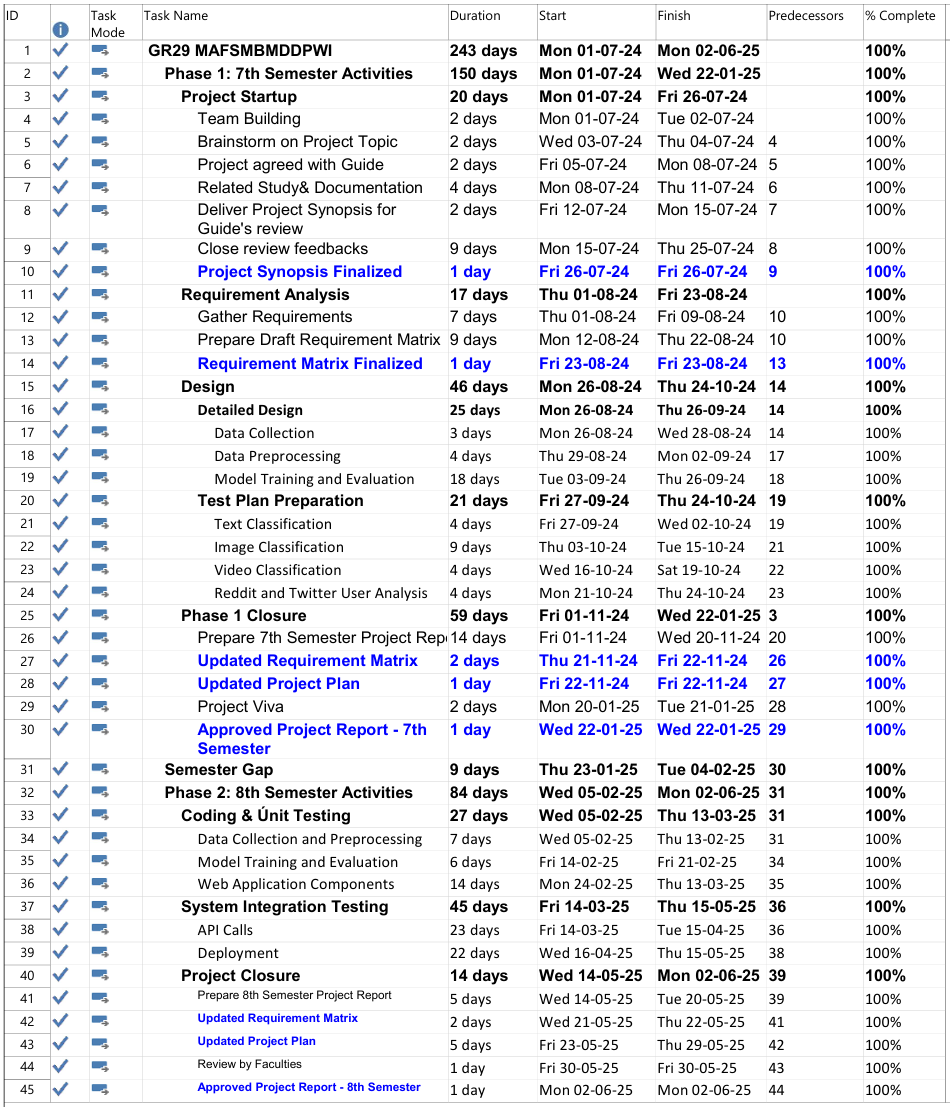
\includegraphics[width=1.0\textwidth]{Images/MS Project Plan Sem 7.png}  
    \caption{Project Plan}
    \label{Project Plan}  % Label for referencing the figure
\end{figure}

\pagebreak

\begin{figure}[h!]  
    \centering
    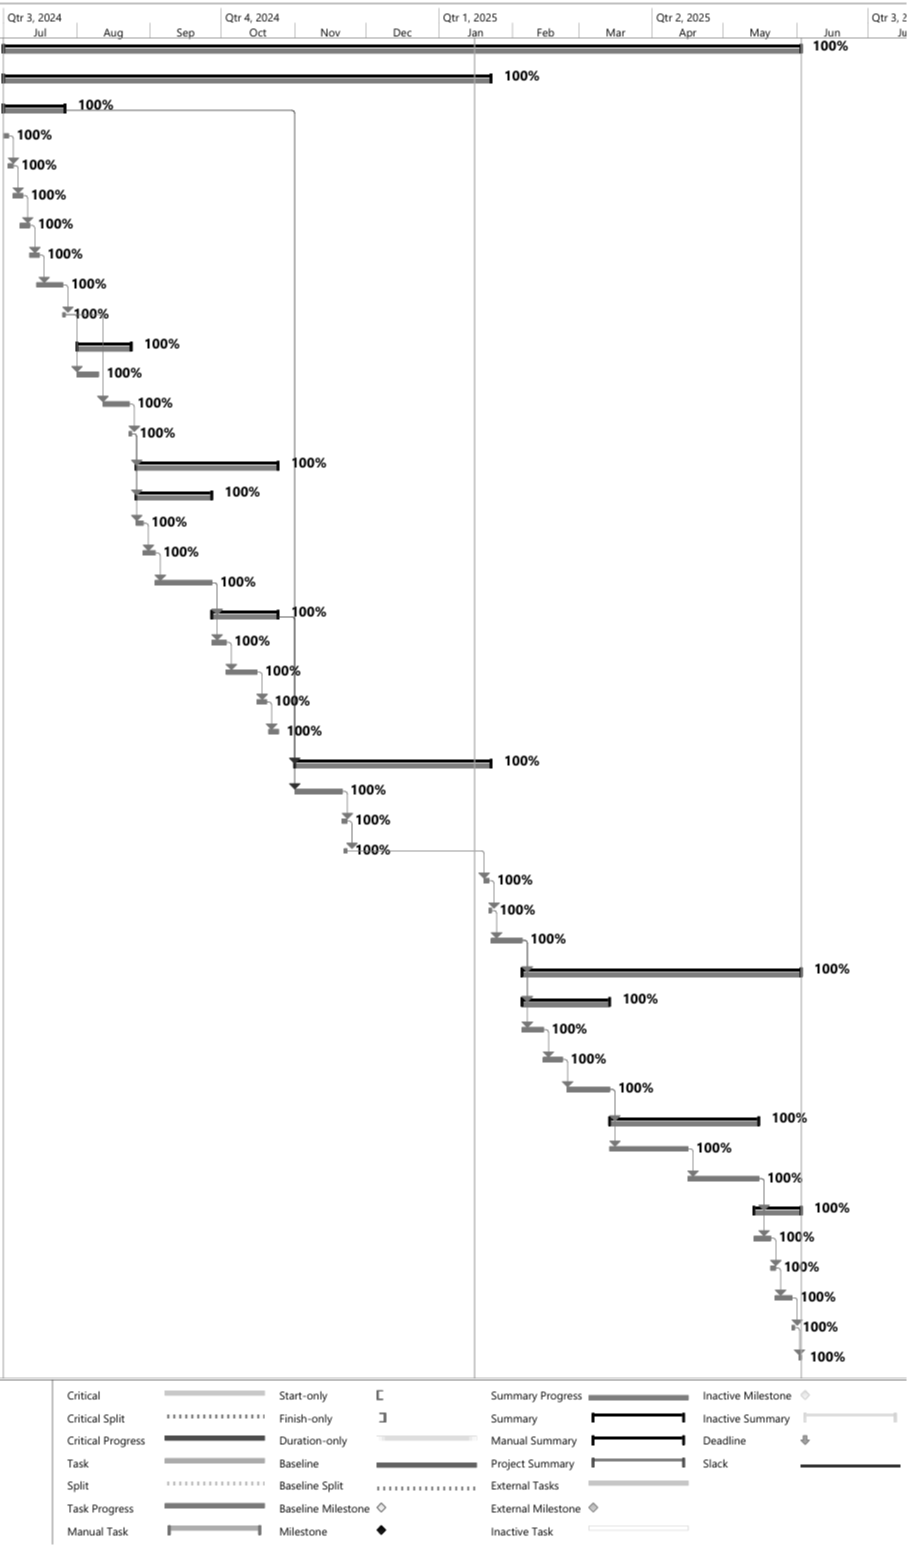
\includegraphics[width=0.79\textwidth]{Images/Gantt Chart.png}  
    \caption{Gantt Chart}
    \label{Gantt Chart}  % Label for referencing the figure
\end{figure}

\pagebreak
% ----------------------- Project Planning ends ------------------------------
